\documentclass[11pt]{article}

% Review mode for anonymous submission
\usepackage[review]{acl}

% Standard packages
\usepackage{times}
\usepackage{latexsym}
\usepackage[T1]{fontenc}
\usepackage[utf8]{inputenc}
\usepackage{microtype}
\usepackage{inconsolata}
\usepackage{graphicx}
\usepackage{booktabs}
\usepackage{amsmath}
\usepackage{multirow}
\usepackage{pifont}
\title{How Gender Bias Enters Clinical Predictions:\\Tracing Shortcut Pathways in Mental Health NLP}

\author{Anonymous ACL submission}

\begin{document}
\maketitle

\begin{abstract}
Mental health classifiers trained on social media text reach high benchmark accuracy, but this performance may rest on \textit{shortcut features}---surface-level writing-style cues spuriously correlated with diagnostic labels through demographic confounds rather than clinical signal. Because women and men write differently, and because several gendered writing styles also correlate with psychopathology, a model can look accurate while in fact keying on gender. Using gender as a case study, we trace how this confound enters predictions. Rather than relabel posts with an explicit gender variable, we decompose gender into 18 interpretable linguistic features---the same surface cues a pretrained encoder actually sees---and introduce a conditional mutual-information test that flags a feature as a gender shortcut when conditioning on gender erases its association with the label. Unlike dataset-level audits, this test isolates confounded features automatically, with no post-hoc domain judgement. Applied across seven diagnostic categories, it flags six condition-invariant gender shortcuts. Probing two pretrained encoders (DistilRoBERTa and MentalRoBERTa), we find every shortcut is linearly recoverable from the frozen [CLS] embedding (AUC $\geq 0.78$), reaches near-peak by Layer~1, and tracks the gender-encoding trajectory rather than the label's. Task fine-tuning \emph{amplifies} gender encoding rather than removing it. Causal mediation shows these shortcuts significantly mediate the gender$\to$label effect (\texttt{fp\_singular} alone $\sim$13.5\%), and embedding-level concept erasure flips 13.8\% of predictions, with a threefold asymmetry against female-authored posts (20.7\% vs.\ 6.8\%). Finally, we close the loop to downstream harm: the fine-tuned classifiers themselves exhibit a large, architecture-independent equalized-odds violation by gender (false-positive-rate gap 0.25, true-positive-rate gap 0.52), false-flagging healthy women roughly five times as often as men. A controlled concept-erasure intervention on the fine-tuned representation causally attributes about half of this disparity to the shortcut subspace---relative to a rank-matched random-erasure control---and shows the remainder collapses when a single gender direction is removed, at modest accuracy cost. Gender-correlated writing style is thus not merely encoded but causally relied upon by deployed classifiers, and the resulting bias is concentrated in a low-dimensional, removable subspace.
\end{abstract}

% ============================================================================
\section{Introduction}

Mental health disorders affect roughly one in eight people worldwide, and NLP systems that detect depression, anxiety, or suicidal ideation from social media text have been proposed to widen access to screening \citep{coppersmith,cohan}. Domain-adapted transformers such as MentalBERT \citep{ji2022mentalbert} and prompted LLMs \citep{xu2024mentalllm,mankarious} report F1 scores of 0.85--0.96 on Reddit benchmarks. Yet high benchmark accuracy can be illusory: models often succeed by exploiting \emph{shortcuts}---surface features correlated with the label in the training data but carrying no causal, clinical meaning \citep{geirhos2020shortcut,mccoy2019right,du2023shortcut}.

In mental health text, the most consequential shortcuts are demographic. Sociolinguistic work shows that women use more first-person singular pronouns, emotional disclosure, and hedging \citep{newman2008gender,schwartz2013personality}, and several of these same features independently correlate with depression \citep{rude2004language}. This creates a gender$\to$writing-style$\to$label confound: a classifier that fires on pronoun density rather than psychopathological content can reach high accuracy while making systematically gender-biased clinical decisions. Whether, and how, pretrained encoders absorb this confound is therefore a prerequisite question for trustworthy mental health NLP.

We study it with gender as a case study. Rather than annotate posts with an explicit gender label and erase it wholesale, we decompose gender into a set of interpretable linguistic features that the sociolinguistics literature establishes as gender-indicative. This lets us observe gender the way an encoder does---indirectly, through writing style---and, crucially, lets us separate gendered signal that is \emph{clinically legitimate} from gendered signal that is a \emph{spurious shortcut}, instead of treating all gender information as something to be removed.

Telling the two apart is exactly where existing tools stop. Dataset auditing frameworks such as G-AUDIT \citep{drenkow2025gaudit} rank features by their mutual information with the label and their recoverability from the input, flagging high-utility, high-detectability features as shortcut risks. This identifies \emph{that} a feature is suspicious, but separating genuine clinical predictors from demographic confounds still requires post-hoc domain expertise, and the audit stops at the dataset. We instead introduce a simple conditional mutual-information test: a feature is a gender shortcut to the extent that conditioning on gender destroys its association with the label ($I(f;Y) \gg I(f;Y\mid G)$). This isolates the confounding pathway directly, needs no clinical judgement about which features ``should'' matter, and, unlike a dataset screen, is carried forward to ask how the flagged shortcuts are represented and how much they actually drive predictions. Concretely, our audit instantiates a staged \emph{detect, locate, quantify} framework, extended with a fourth \emph{measure-harm} stage, that follows one interpretable feature set from the dataset into the deployed model's decisions.

\paragraph{Research questions.}
\begin{itemize}
\setlength\itemsep{0pt}
\item[\textbf{RQ1}] Which writing-style features function as gender-mediated shortcuts for mental health classification, and are they shortcut-like across diagnostic conditions?
\item[\textbf{RQ2}] Are these shortcuts encoded in pre-trained transformer representations, at what depth, and is encoding stable across model architecture and pretraining domain?
\item[\textbf{RQ3}] How much of the gender$\to$prediction pathway flows through identifiable shortcuts, and is the reliance gender-asymmetric?
\item[\textbf{RQ4}] Does task fine-tuning amplify or attenuate shortcut and gender encoding?
\item[\textbf{RQ5}] Do the encoded shortcuts cause measurable downstream harm---a gender disparity in deployed classifiers' decisions---and does a targeted intervention on the shortcut subspace reduce it?
\end{itemize}

\paragraph{Contributions.}
We present:
(1)~a conditional mutual-information shortcut test, calibrated by a gender-permutation null, that flags 6 condition-invariant gender shortcuts across 7 diagnostic categories without requiring domain expertise;
(2)~layer-wise probing across DistilRoBERTa-base (6 layers) and MentalRoBERTa (12 layers, domain-pretrained), showing shortcuts are encoded from Layer~1 in both architectures and track gender more than the label;
(3)~a fine-tuning comparison showing that \emph{supervised fine-tuning amplifies gender encoding} in both DistilRoBERTa and MentalRoBERTa, and that domain pretraining does not reduce shortcut reliance;
(4)~causal mediation and concept-erasure analyses quantifying the gender$\to$label pathway through shortcuts (\texttt{fp\_singular} mediates $\sim$13.5\%; erasing all shortcuts flips 13.8\% of predictions) and exposing a $3\times$ asymmetry against female-authored posts; and
(5)~a model-level harm result closing the encoding$\to$use$\to$harm chain---the fine-tuned classifiers show a large, architecture-independent equalized-odds violation by gender (FPR gap 0.25, TPR gap 0.52), and a controlled concept-erasure intervention attributes about half of it to the shortcut subspace (vs.\ a random-erasure control) and nearly all of it to a single removable gender direction.

% ============================================================================
\section{Related Work}

\paragraph{Shortcut learning in NLP.}
Shortcut learning occurs when models exploit statistical regularities correlated with labels but not causally related to the task \citep{geirhos2020shortcut}.
NLI models exploit lexical overlap \citep{mccoy2019right}, sentiment classifiers learn author identity, and toxicity detectors fire on identity-group mentions.
\citet{du2023shortcut} survey shortcut learning in LLMs across NLU tasks.
Mitigation strategies include Product-of-Experts ensembles \citep{clark2020poe} and counterfactual data augmentation, but none have been applied to mental health NLP.

\paragraph{Dataset-level bias auditing.}
G-AUDIT \citep{drenkow2025gaudit} proposes a modality-agnostic dataset auditing framework that uses mutual information to rank attributes by their \emph{utility} ($\text{MI}(A;Y)$) and \emph{detectability} ($\text{MI}(A;\hat{A})$), flagging those in the upper-right quadrant as shortcut risks. Their framework answers a screening question: \emph{which attributes are both associated with the label and recoverable from the input?} This is a broad, portable test, but it stops at correlation---distinguishing genuine predictors from spurious ones requires post-hoc domain expertise. Our work answers a fundamentally different question: \emph{how much of a feature's predictive power is mediated by a specific protected attribute?} By comparing $I(f;Y)$ against $I(f;Y \mid G)$, we directly isolate the confounding mechanism rather than flagging co-occurrence, producing a shortcut diagnosis that is causal in nature rather than associational.

\paragraph{Gender, language, and mental health NLP.}
Women use more first-person singular pronouns, emotional disclosure, and hedging \citep{newman2008gender,schwartz2013personality}---features also correlated with depression \citep{rude2004language}---creating a confound.
MentalBERT \citep{ji2022mentalbert} degrades substantially when topic words are removed, suggesting lexical reliance.
\citet{harrigian2023characterization} showed mental health classifiers exploit demographic proxies; \citet{schuller2025bias} found gender shifts classification outcomes in multilingual settings.
Yet the \textit{mechanism} by which gender-correlated features mediate predictions has not been traced at the feature level.

\paragraph{Probing and causal methods.}
Probing classifiers \citep{belinkov2022probing} test whether properties are linearly encoded in representations, and concept-erasure methods such as INLP \citep{ravfogel2020null} remove a target direction to measure its effect on downstream predictions.
Causal mediation analysis \citep{imai2010general} decomposes effects into direct and indirect components; \citet{vig2020mediation} applied it to GPT-2 attention heads.
These tools have been applied individually but not combined into a systematic, cross-architecture shortcut audit for mental health representations.

% ============================================================================
\section{Data}

\paragraph{Dataset.}
We use a curated subset of the Mindset corpus \citep{koloski2024mindset} (Reddit mental health and control subreddits), with binary gender labels from high-precision regex matching on explicit self-disclosure (e.g., ``I'm a 24F'').
Table~\ref{tab:data} summarises the dataset.

\begin{table}[t]
\centering
\small
\caption{Dataset characteristics.}
\label{tab:data}
\begin{tabular}{ll}
\toprule
\textbf{Property} & \textbf{Value} \\
\midrule
Total posts & 32,200 \\
Male / Female & 16,100 / 16,100 \\
Control / MH-positive & 22,601 / 9,599 \\
Female positive rate & 43.0\% \\
Male positive rate & 16.8\% \\
\bottomrule
\end{tabular}
\end{table}

The $2.6\times$ gap in positive rates creates the conditions under which gender-mediated shortcut learning is most likely to occur, making this dataset well suited to auditing.

\paragraph{Linguistic features.}
We represent each post with 18 interpretable, open-lexicon linguistic features. Their selection is deliberately grounded in the clinical and psycholinguistic literature on how language reflects both gender and mental state: first-person pronoun use, emotional and negative-affect language, hedging, absolutist and certainty terms, and body/health references are all documented markers of depression and related conditions \citep{coppersmith,cohan,rude2004language,almosaiwi2018absolutist} that are also gendered in their distribution \citep{newman2008gender,schwartz2013personality,park2016women}. We reimplement these dimensions as transparent open word lists in the spirit of---but not dependent on---the proprietary LIWC framework \citep{tausczik2010liwc}, computing each feature as a normalized token-count density or a log-transformed count. The full inventory, with a per-feature clinical justification and citations, is given in Appendix~\ref{sec:features}.

Four of the 18 features (\texttt{analytic}, \texttt{self\_ref\_rumination}, \texttt{cogproc}, \texttt{clout}) are included as clinically-grounded reference features: they are gender-correlated yet carry genuine clinical signal, so a well-behaved shortcut test should largely leave them unflagged. They provide a built-in selectivity check for the test introduced next (\S\ref{sec:mi-decomposition}).

% ============================================================================
\section{Methods}

Our analysis follows one feature set from data to predictions: we first \emph{detect} which linguistic features act as gender-mediated shortcuts (RQ1), then \emph{locate} where those shortcuts are encoded in pretrained representations and how fine-tuning changes them (RQ2, RQ4), \emph{quantify} how much of the gender$\to$prediction pathway flows through them (RQ3), and finally \emph{measure} the resulting downstream harm in deployed classifiers and intervene on it (RQ5).

\subsection{Detecting gender-mediated shortcuts}

\paragraph{Single-feature predictive power.}
For each of the 18 features we train a logistic regression classifier (5-fold stratified CV) to predict the binary label using that feature alone, recording the AUC. This measures raw predictive power but, on its own, cannot tell genuine clinical signal from gender confounding---the question the next test addresses.

\paragraph{Conditional mutual-information test.}
\label{sec:mi-decomposition}

To separate gender-confounded shortcuts from genuinely predictive features, we ask how much of the information a feature shares with the label \emph{survives} once gender is held fixed. For each feature $f$, we compute three quantities using the $k$-nearest-neighbour MI estimator of \citet{kraskov2004estimating} (implemented via \texttt{sklearn}, $k{=}5$):
\begin{align}
    I(f;\, Y)         &\quad \label{eq:mi-label} \\
    I(f;\, G)         &\quad  \label{eq:mi-gender} \\
    I(f;\, Y \mid G)  &= \textstyle\sum_{g} P(G{=}g)\; I(f;\, Y)_{G=g} \quad \label{eq:mi-cond}
\end{align}
The conditional MI in~\eqref{eq:mi-cond} is computed by stratifying the data into male and female subsets, estimating $I(f; Y)$ within each stratum, and taking the weighted average. This follows directly from the chain rule of mutual information~\citep{cover2006elements} and avoids the need for explicit density estimation of the joint distribution $P(f, Y, G)$.

The \textbf{MI drop} for feature $f$ is defined as
\begin{equation}
    \Delta_f = I(f;\, Y) - I(f;\, Y \mid G),
    \label{eq:mi-drop}
\end{equation}
which quantifies the portion of $f$'s label-predictive information that is mediated by gender. A large positive $\Delta_f$ indicates that much of $f$'s apparent clinical signal is explained by the confounding path $f \leftarrow G \rightarrow Y$ rather than the direct path $f \rightarrow Y$. This is the crux of the test: it singles out gender-confounded features automatically, without any prior judgement about which features ``ought'' to be clinically meaningful---the post-hoc domain expertise that a dataset-level utility/detectability screen \citep{drenkow2025gaudit} still requires.

\paragraph{Permutation calibration.}
Rather than relying on an ad-hoc threshold for $\Delta_f$, we calibrate significance using a permutation test. Under the null hypothesis $H_0{:}$ gender labels are independent of the feature--label relationship, we:
\begin{enumerate}
    \item Randomly permute the gender vector $\mathbf{g}$ (breaking any true $f$--$G$ association).
    \item Recompute $I(f;\, Y \mid G^{\pi})$ using the permuted gender assignments.
    \item Record the null MI drop $\Delta_f^{\pi} = I(f;\, Y) - I(f;\, Y \mid G^{\pi})$.
\end{enumerate}
We repeat this $B{=}200$ times per condition to build a null distribution of MI drops. The permutation $p$-value is
\begin{equation}
    p_f = \frac{1}{B} \sum_{b=1}^{B} \mathbf{1}\!\left[\Delta_f^{(\pi_b)} \geq \Delta_f^{\text{obs}}\right].
\end{equation}
A feature is flagged as a \textbf{gender shortcut} if $p_f < 0.05$. This approach is preferable to a fixed percentage threshold (e.g., 20\% MI drop) because the null distribution automatically accounts for estimation noise, sample size, and the base-rate gender imbalance in each condition---all of which vary across the seven diagnostic categories in our data.

The permutation test is a standard nonparametric calibration strategy for MI-based statistics where the sampling distribution is analytically intractable~\citep{roulston1999estimating,steuer2002mutual}. By permuting gender rather than labels, we specifically test whether the observed MI drop is attributable to genuine gender--feature dependence or merely to finite-sample noise in the stratified MI estimate.

\paragraph{Cross-condition analysis.}
We apply this procedure independently to each of the seven conditions in the dataset (ADHD, anxiety, autism, bipolar disorder, depression, OCD, PTSD), each balanced against the shared control group, producing the feature $\times$ condition shortcut matrix in Table~\ref{tab:cross-condition}. A feature flagged across multiple conditions is a \emph{condition-invariant} gender confound, a systematic property of the feature rather than a condition-specific artefact, and we define a \textbf{condition-invariant gender shortcut} as one flagged in $\geq 2/7$ conditions. The four reference features provide a selectivity check: a test that flagged every predictive feature would flag them too. In downstream analyses we treat the six flagged \emph{candidate} features as shortcuts and the four \emph{reference} features as controls. The test does additionally flag two reference features (\texttt{analytic}, \texttt{self\_ref\_rumination}), consistent with their documented gendering; this is expected behaviour for a gender-confound detector, and we retain them as reference features for comparison rather than reclassifying them.
\begin{table*}[t]
\centering
\small
\caption{Cross-condition gender shortcut matrix. Each cell indicates whether the feature was flagged as a significant gender shortcut ($p < 0.05$, permutation test, 200 shuffles). {\ding{51}} = flagged; {\large$\star$} marks control features. Features sorted by number of conditions flagged.}
\label{tab:cross-condition}
\begin{tabular}{@{}l ccccccc c l@{}}
\toprule
Feature & ADHD & Anx. & Aut. & Bip. & Dep. & OCD & PTSD & $n$/7 & Role \\
\midrule
\texttt{fp\_singular}           & \ding{51} & \ding{51} & \ding{51} & \ding{51} & \ding{51} & \ding{51} & \ding{51} & 7 & Candidate \\
\texttt{analytic}$\,\star$      & \ding{51} & \ding{51} &           & \ding{51} & \ding{51} & \ding{51} & \ding{51} & 6 & Control \\
\texttt{body\_health}           & \ding{51} & \ding{51} & \ding{51} & \ding{51} & \ding{51} & \ding{51} &           & 6 & Candidate \\
\texttt{post\_length}           & \ding{51} &           & \ding{51} & \ding{51} & \ding{51} &           &           & 4 & Candidate \\
\texttt{self\_ref\_rum.}$\,\star$ &         & \ding{51} &           & \ding{51} & \ding{51} &           &           & 3 & Control \\
\texttt{hedge\_density}         & \ding{51} &           &           &           &           & \ding{51} &           & 2 & Candidate \\
\texttt{negative\_emotion}      &           & \ding{51} &           & \ding{51} &           &           &           & 2 & Candidate \\
\texttt{emotional\_feeling}     &           &           &           & \ding{51} &           & \ding{51} &           & 2 & Candidate \\
\texttt{social\_relational}     &           &           &           & \ding{51} &           &           &           & 1 & Candidate \\
\texttt{cogproc}$\,\star$       & \ding{51} &           &           &           &           &           &           & 1 & Control \\
\texttt{anger}                  &           &           &           &           &           &           &           & 0 & Candidate \\
\texttt{apology\_selfblame}     &           &           &           &           &           &           &           & 0 & Candidate \\
\texttt{certainty}              &           &           &           &           &           &           &           & 0 & Candidate \\
\texttt{clout}$\,\star$         &           &           &           &           &           &           &           & 0 & Control \\
\texttt{excl\_intensifiers}     &           &           &           &           &           &           &           & 0 & Candidate \\
\texttt{fp\_plural}             &           &           &           &           &           &           &           & 0 & Candidate \\
\texttt{question\_density}      &           &           &           &           &           &           &           & 0 & Candidate \\
\texttt{swear\_words}           &           &           &           &           &           &           &           & 0 & Candidate \\
\bottomrule
\end{tabular}
\end{table*}

\subsection{Locating shortcuts in representations}

\paragraph{Choice of models.}
If gender shortcuts are encoded by only one model, the problem is an idiosyncrasy of that pretraining recipe; if they appear across models that differ in the dimensions usually credited for representation quality, the problem lies in the data. We therefore select two encoders that isolate the two dimensions most often credited in mental health NLP, model depth/capacity and pretraining domain:
\begin{itemize}
\setlength\itemsep{0pt}
\item \textbf{DistilRoBERTa-base} (82M params, 6 layers, BPE tokenizer, MLM pretraining, generic web corpus): a minimal-capacity baseline that isolates \emph{depth}.
\item \textbf{MentalRoBERTa} \citep{ji2022mentalbert} (125M params, 12 layers, BPE, MLM, \emph{pretrained on Reddit mental-health posts}): isolates the effect of in-\emph{domain} pretraining, the standard recommendation for this task.
\end{itemize}
For each model we audit two regimes: (i) the \textbf{frozen} pretrained encoder (no task adaptation), and (ii) a \textbf{task-fine-tuned} encoder, obtained by training a sequence classification head on $\text{text} \to \text{binary\_label}$ (80/20 stratified split, 3 epochs, AdamW with warmup, best epoch by validation AUC). All probing is performed on the encoder body only, with the classification head discarded before extraction, so that frozen and fine-tuned representations are directly comparable. This yields four audited model$\times$regime cells in total.

\paragraph{Final-layer probing.}
For each shortcut, control, gender, and the binary label, we train logistic probing classifiers (5-fold stratified CV) on the final-layer [CLS] embeddings of each model$\times$regime. We report both continuous regression $R^2$ (Ridge) and median-split AUC, on a common 32{,}200-row set.

\paragraph{Layer-wise probing.}
To trace \textit{when} shortcuts are encoded, we extract [CLS] from every extraction point of both models (DistilRoBERTa: embedding + 6 transformer layers = 7; MentalRoBERTa: embedding + 12 = 13) and repeat the probing protocol at each depth. We compare shortcut, gender, and label curves to test whether shortcuts track the gender or the label encoding trajectory.

\subsection{Quantifying reliance on shortcuts}

Detecting a shortcut and finding it encoded does not establish that predictions \emph{depend} on it. We quantify dependence two complementary ways: causal mediation at the \textit{linguistic-feature level}, which characterises the dataset and so applies to every model, and concept erasure at the \textit{embedding level}, reported on the frozen DistilRoBERTa representation.

\paragraph{Causal mediation analysis.}
Following \citet{imai2010general}, for each shortcut $M$ we estimate the Average Causal Mediation Effect (ACME, $G \to M \to Y$), the Average Direct Effect (ADE, $G \to Y$ not through $M$), and the proportion mediated, with 1{,}000 bootstrap replications for 95\% CIs. The structural causal model posits $G \to S \to E \to \hat{Y}$ (shortcut path) alongside $G \to C \to E \to \hat{Y}$ (clinical signal path) and a potential direct path $G \to \hat{Y}$.

\paragraph{Concept erasure and counterfactual prediction flips.}
To complement the feature-level mediation analysis with a representation-level intervention, we apply Iterative Nullspace Projection \citep{ravfogel2020null} to the frozen DistilRoBERTa [CLS] embeddings: for each shortcut, we erase its linearly recoverable component (rank up to 15) and measure (a) the AUC drop of an embedding-level classifier targeting the shortcut concept (verifying erasure), (b) the AUC drop of a label classifier (estimating how much the label rides on the shortcut subspace), and (c) the fraction of predictions whose binary label \emph{flips} after erasure. We stratify flips by gender to recover the asymmetry that ablation in feature space leaves implicit. We also erase the gender direction itself as a reference point.

\paragraph{Feature ablation.}
A complementary linguistic-feature ablation---measuring AUC of the full 18-feature model after zeroing each shortcut individually and all 8 simultaneously, with gender-stratified deltas---is reported in Appendix~\ref{sec:ablation}.

\subsection{Measuring and intervening on downstream harm}
\label{sec:methods-harm}

Encoding and mediation establish that shortcuts are present and partly drive the \emph{dataset}-level gender$\to$label association; neither shows that a \emph{deployed} model's decisions are harmed. We close this with two analyses on the fine-tuned classifiers themselves, evaluated only on the held-out validation split (the 20\% of posts never seen during fine-tuning).

\paragraph{Group fairness of decisions.}
For each fine-tuned classifier we threshold its predicted positive-class probability at 0.5 and compute by-gender group-fairness metrics with \texttt{fairlearn} \citep{bird2020fairlearn}: the false-positive-rate (FPR) and true-positive-rate (TPR) gaps, the equalized-odds difference \citep{hardt2016equality}, per-group selection rate, and per-group AUC. We attach 2{,}000-resample bootstrap 95\% CIs and a 2{,}000-permutation null over the gender labels. Because the male and female base rates differ sharply (Table~\ref{tab:data}), we lead with equalized odds---which conditions on the true label and is not licensed by base-rate differences---and explicitly decompose the gap against the calibration/base-rate confound \citep{chouldechova2017fair,kleinberg2017inherent} via group calibration and group-equalized thresholds.

\paragraph{Causal fairness intervention.}
To test whether the disparity is \emph{carried by} the shortcut subspace, we erase that subspace from the fine-tuned [CLS] vector and run the \emph{unchanged} classification head on the erased representation (the head reproduces the model's logits exactly, so the intervention is exact). Erasure uses LEACE \citep{belrose2023leace}, the minimal-norm linear edit that renders a target concept linearly unpredictable. Fitting all projections on the training split and measuring the gap on validation, we compare four conditions: \textbf{baseline} (no erasure); \textbf{shortcut-erase} (the 8-feature subspace); \textbf{gender-erase} (the binary-gender direction---a ceiling); and \textbf{random-erase} (a rank-matched random subspace, averaged over 10 seeds)---the control that separates a specific causal pathway from the generic effect of deleting representational dimensions. We track overall label AUC (collateral damage) and post-erasure gender decodability (erasure validity).

% ============================================================================
\section{Results}
\label{sec:results}

\subsection{Shortcut detection}

Individual feature AUCs in a single-feature logistic model range from $\sim$0.50 (\texttt{question\_density}, \texttt{swear\_words}) to 0.64 (\texttt{fp\_singular}); the combined 18-feature logistic baseline reaches AUC $= 0.721 \pm 0.007$. The cross-condition permutation test (Table~\ref{tab:cross-condition}) flags six candidate features as condition-invariant gender shortcuts, led by \texttt{fp\_singular}, the only feature flagged in all 7/7 conditions. The test is selective rather than indiscriminate: ten of the eighteen features are never flagged in two or more conditions. Among the four reference features, \texttt{clout} (0/7) and \texttt{cogproc} (1/7) remain unflagged as intended, while \texttt{analytic} (6/7) and \texttt{self\_ref\_rumination} (3/7) are flagged, consistent with the sociolinguistic record that both are gendered; we retain all four as reference features and carry the six flagged candidates forward as shortcuts.

\subsection{Representation probing}

\paragraph{Final-layer probing across models.}
Both audited models encode the 6 shortcuts at high recoverability from their frozen [CLS] (Table~\ref{tab:probing-multi}). Probe AUCs are $\geq 0.78$ for every shortcut in both models, with \texttt{post\_length} essentially perfect ($>0.99$). Gender is encoded at AUC $\geq 0.948$ in both frozen models, and after task fine-tuning gender encoding \emph{increases further} (DistilRoBERTa $0.959 \to 0.984$; MentalRoBERTa $0.948 \to 0.980$), the opposite of what one might expect if supervised training pulled the representation toward the diagnostic outcome and away from demographic surface cues.

\begin{table}[t]
\centering
\small
\caption{Final-layer probing AUC across audited model$\times$regime cells. Each cell is the median-split classification AUC of a 5-fold logistic probe over the 32,200-post corpus. ``Fr.'' $=$ frozen pretrained encoder; ``FT'' $=$ task-fine-tuned encoder (encoder body only). The six shortcuts are in the top block, the four reference features below the first rule, and gender/label below the second. \textbf{Bold} cells indicate AUC $\geq 0.95$; \textit{italic} cells indicate gender or label AUC. The test flags \texttt{analytic} and \texttt{self\_ref\_rumination} as gendered but we retain them as reference features (\S\ref{sec:results}).}
\label{tab:probing-multi}
\begin{tabular}{@{}l cc cc@{}}
\toprule
& \multicolumn{2}{c}{\textbf{DistilRoBERTa}} & \multicolumn{2}{c}{\textbf{MentalRoBERTa}} \\
\cmidrule(lr){2-3}\cmidrule(lr){4-5}
Probe target & Fr. & FT & Fr. & FT \\
\midrule
\texttt{fp\_singular}      & \textbf{0.976} & \textbf{0.953} & \textbf{0.968} & 0.948 \\
\texttt{body\_health}      & 0.885 & 0.869 & 0.877 & 0.856 \\
\texttt{post\_length}      & \textbf{0.998} & \textbf{0.994} & \textbf{0.995} & \textbf{0.989} \\
\texttt{hedge\_density}    & 0.832 & 0.781 & 0.829 & 0.779 \\
\texttt{negative\_emotion} & 0.895 & 0.877 & 0.888 & 0.871 \\
\texttt{emotional\_feel.}  & 0.859 & 0.816 & 0.852 & 0.810 \\
\midrule
\texttt{analytic} (ref)    & 0.932 & 0.884 & \textbf{0.933} & 0.892 \\
\texttt{self\_ref\_rum.} (ref) & 0.908 & 0.892 & 0.901 & 0.887 \\
\texttt{cogproc} (ref)     & 0.887 & 0.839 & 0.883 & 0.848 \\
\texttt{clout} (ref)       & 0.943 & 0.889 & \textbf{0.932} & 0.904 \\
\midrule
\textit{Gender}            & \textbf{\textit{0.959}} & \textbf{\textit{0.984}} & \textit{0.948} & \textbf{\textit{0.980}} \\
\textit{Binary label}      & \textit{0.798} & \textit{0.832} & \textit{0.806} & \textit{0.865} \\
\bottomrule
\end{tabular}
\end{table}

\paragraph{Layer-wise probing.}
Figure~\ref{fig:layerwise} shows probing AUC at each extraction point of frozen DistilRoBERTa (embedding + 6 transformer layers). All shortcut features jump from chance ($\sim$0.50) to near-peak AUC at Layer~1 and stay flat thereafter. Gender follows the same trajectory (0.953 at L1, U-shaped dip to 0.934 at L5, recovery to 0.959 at L6). The binary label, by contrast, builds slowly ($0.780 \to 0.798$). The same Layer-1-peak pattern holds for MentalRoBERTa (gender 0.956 at L1, 0.947 at L12). The alignment of shortcut curves with the gender curve, and their dissociation from the label's gradual build-up, supports the view that shortcuts encode demographic surface signal, not clinical content.

\begin{figure}[t]
\centering
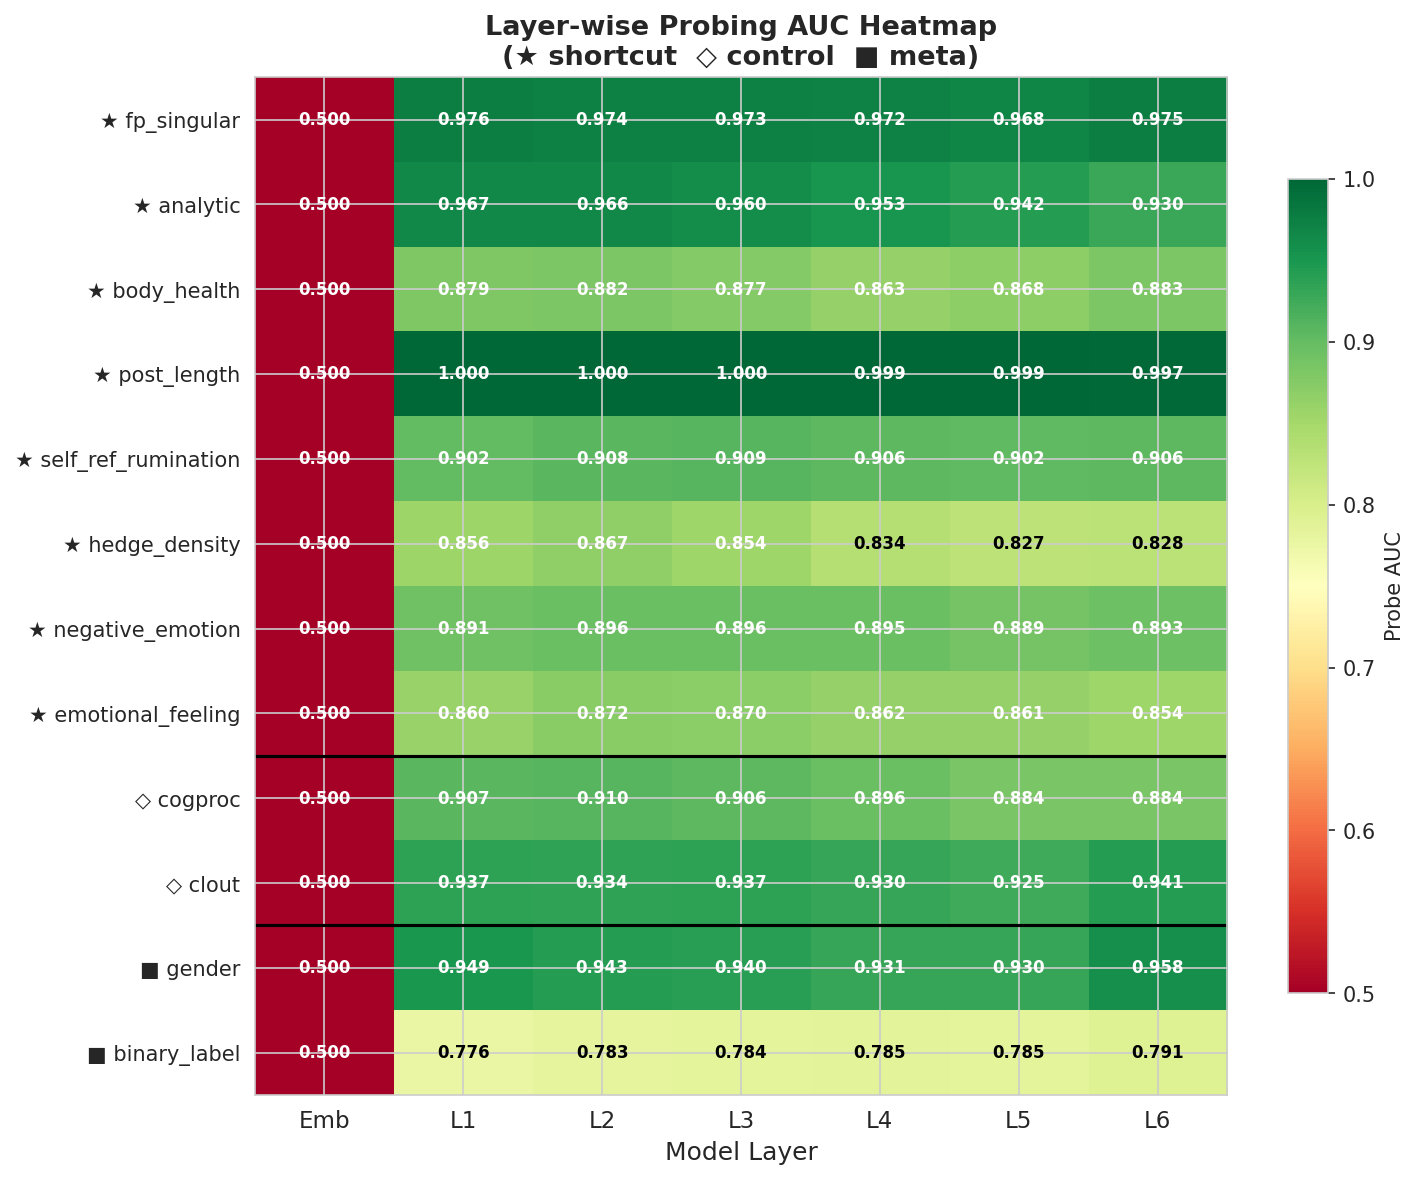
\includegraphics[width=\columnwidth]{data/stage2/layerwise_heatmap.png}
\caption{Layer-wise probing AUC for shortcuts, gender, and label across 7 DistilRoBERTa extraction points. Shortcuts reach near-peak at Layer~1 and track the gender curve; the label builds gradually.}
\label{fig:layerwise}
\end{figure}

\paragraph{Fine-tuning effect.}
Comparing frozen and fine-tuned columns in Table~\ref{tab:probing-multi}: most shortcut probing AUCs decrease modestly after fine-tuning (e.g., DistilRoBERTa \texttt{fp\_singular} $0.976 \to 0.953$; MentalRoBERTa \texttt{emotional\_feeling} $0.852 \to 0.810$), yet gender AUC \emph{rises} in both models (DistilRoBERTa $+0.025$; MentalRoBERTa $+0.032$), and label AUC also rises ($+0.034$ and $+0.059$ respectively). Fine-tuning does not flush demographic signal out of the encoder; it consolidates it.

\subsection{Reliance on shortcuts}

\paragraph{Causal mediation.}
The total gender $\to$ label effect is $+0.259$ on the probability scale (females are $\sim$26 pp more likely to receive a positive label under the dataset's base rates). Five of the eight shortcuts have completed bootstrap mediation analyses (Table~\ref{tab:mediation}); all are statistically significant mediators with 95\% bootstrap CIs strictly excluding zero. \texttt{fp\_singular} alone mediates 13.5\% of the total effect (ACME $= +0.035$, 95\% CI $[+0.032, +0.038]$). The five quantified shortcuts together account for $\sim$26\% of the indirect path; the remainder flows through the three not-yet-quantified shortcuts and other unmeasured channels.

\begin{table}[t]
\centering
\small
\caption{Causal mediation results (1{,}000 bootstrap replications). All entries significant at $p < 0.05$ (CI excludes zero). Mediation for \texttt{analytic}, \texttt{body\_health}, and \texttt{self\_ref\_rumination} is pending; total mediated $\geq$26\% should be read as a lower bound.}
\label{tab:mediation}
\begin{tabular}{lccc}
\toprule
\textbf{Feature} & \textbf{ACME} & \textbf{95\% CI} & \textbf{Prop.} \\
\midrule
\texttt{fp\_singular}       & $+0.035$ & {$[+.032, +.038]$} & 13.5\% \\
\texttt{emotional\_feeling} & $+0.013$ & {$[+.012, +.015]$} &  5.2\% \\
\texttt{negative\_emotion}  & $+0.011$ & {$[+.009, +.012]$} &  4.1\% \\
\texttt{post\_length}       & $+0.007$ & {$[+.005, +.008]$} &  2.6\% \\
\texttt{hedge\_density}     & $+0.002$ & {$[+.001, +.003]$} &  0.8\% \\
\midrule
\textit{Sum (quantified)}   &          &                   & \textit{$\geq$26.2\%} \\
\bottomrule
\end{tabular}
\end{table}

\paragraph{Concept erasure and counterfactual flips.}
INLP applied to frozen DistilRoBERTa [CLS] removes the linearly recoverable direction of each shortcut (verified: concept-probe AUC drops by 0.03--0.09 per shortcut) while leaving the embedding-level label AUC essentially unchanged ($\Delta_{\text{label AUC}} \in [-0.0005, -0.0001]$). The label signal therefore does not ride on the recoverable shortcut directions in any large-scale linear sense---but \emph{individual predictions still depend on them}: erasing a single shortcut flips 1.3--9.4\% of binary predictions, and erasing all 8 simultaneously flips 13.8\% (Table~\ref{tab:erasure}). The flips are sharply gender-asymmetric: female-authored posts flip 2--3$\times$ more often than male-authored posts. Erasing all shortcuts flips 20.7\% of female predictions vs.\ 6.8\% of male predictions (asymmetry $+13.8$ pp), and a direct gender-direction erasure flips 14.6\% female vs.\ 5.4\% male predictions.

\begin{table}[t]
\centering
\small
\caption{Counterfactual prediction flips after INLP concept erasure on frozen DistilRoBERTa [CLS]. ``Flip'' is the fraction of posts whose predicted label changes; ``M/F'' are gender-stratified; ``Asym.''~$=$ F$-$M.}
\label{tab:erasure}
\begin{tabular}{lcccc}
\toprule
\textbf{Erase} & \textbf{Flip} & \textbf{M} & \textbf{F} & \textbf{Asym.} \\
\midrule
\texttt{emotional\_feeling}    &  9.4\% & 4.7\% & 14.1\% & $+9.4$ \\
\texttt{negative\_emotion}     &  8.5\% & 4.4\% & 12.5\% & $+8.2$ \\
\texttt{post\_length}          &  6.9\% & 3.6\% & 10.2\% & $+6.6$ \\
\texttt{hedge\_density}        &  3.0\% & 1.7\% &  4.2\% & $+2.4$ \\
\texttt{fp\_singular}          &  1.9\% & 1.1\% &  2.8\% & $+1.7$ \\
\midrule
All 8 shortcuts                & 13.8\% & 6.8\% & 20.7\% & $+13.8$ \\
Gender direction               & 10.0\% & 5.4\% & 14.6\% & $+9.2$ \\
\bottomrule
\end{tabular}
\end{table}

The fact that all-shortcut erasure produces \emph{more} flips---and stronger female asymmetry---than gender erasure itself indicates that the model's gender reliance is distributed across multiple shortcut directions rather than concentrated in a single demographic axis. Erasure of any one shortcut closes only a small fraction of the gender gap.

\subsection{Downstream harm and causal intervention}
\label{sec:harm}

Encoding, mediation, and embedding-level erasure all stop short of the deployed model's decisions. We now show those decisions are gender-disparate, and that the disparity is causally carried by the shortcut subspace.

\paragraph{Group fairness of classifier decisions.}
On the held-out validation split (6{,}440 posts; female MH base rate 41.6\%, male 18.0\%), both fine-tuned classifiers exhibit a large equalized-odds violation \citep{hardt2016equality} (Table~\ref{tab:fairness}). At the default 0.5 threshold, DistilRoBERTa-FT predicts the positive class for 50.4\% of women but only 9.4\% of men; its false-positive rate is five times higher for women (0.315 vs.\ 0.060; gap $+0.254$) and its true-positive-rate gap is $+0.519$. MentalRoBERTa-FT is near-identical, and all gaps are significant (gender-permutation $p<0.0005$; e.g.\ bootstrap 95\% CI for the FPR gap $[+0.232,+0.276]$). In deployment terms, the classifier false-flags roughly one in three healthy women as mental-health-positive while detecting only one in four genuinely affected men.

We stress-test this against the standard objection that unequal base rates mechanically induce FPR/TPR gaps at a fixed threshold \citep{chouldechova2017fair,kleinberg2017inherent}. Two components survive it. The by-group \emph{AUC} gap ($+0.055$/$+0.059$; men are ranked worse) is threshold-free, and the classifier is asymmetrically \emph{mis-calibrated}---over-predicting the positive class for women by $\sim$6 pp beyond their (already higher) base rate while remaining calibrated for men (amplification, not base-rate tracking). We therefore report the deployment-threshold gap as the \emph{operational} harm and the AUC gap plus over-prediction as its base-rate-robust core, without overclaiming the full $0.52$ as model bias.

\begin{table}[t]
\centering
\small
\caption{Group fairness of the fine-tuned classifiers on the held-out split, at threshold 0.5. ``Gap'' is Female$-$Male. All gaps significant at permutation $p<0.0005$. The FPR/TPR gaps reflect a deployment-threshold disparity; the AUC gap is threshold-free.}
\label{tab:fairness}
\begin{tabular}{@{}l ccc c ccc@{}}
\toprule
& \multicolumn{3}{c}{\textbf{DistilRoBERTa-FT}} && \multicolumn{3}{c}{\textbf{MentalRoBERTa-FT}}\\
\cmidrule(lr){2-4}\cmidrule(lr){6-8}
& F & M & Gap && F & M & Gap\\
\midrule
FPR       & 0.315 & 0.060 & $+.254$ && 0.304 & 0.051 & $+.253$\\
TPR       & 0.770 & 0.251 & $+.519$ && 0.765 & 0.246 & $+.519$\\
Selection & 0.504 & 0.094 & $+.410$ && 0.496 & 0.086 & $+.410$\\
AUC       & 0.794 & 0.739 & $+.055$ && 0.808 & 0.749 & $+.059$\\
\bottomrule
\end{tabular}
\end{table}

\paragraph{Causal fairness intervention.}
Erasing the shortcut subspace from the fine-tuned representation and re-running the unchanged classification head roughly halves the equalized-odds violation (DistilRoBERTa $0.519 \to 0.272$, $-48\%$; MentalRoBERTa $0.519 \to 0.284$; Table~\ref{tab:intervention}, Figure~\ref{fig:intervention}). The rank-matched random-erasure control leaves it essentially intact ($0.519 \to 0.507 \pm 0.008$), so the reduction is specific to the shortcut directions rather than a generic effect of removing eight dimensions---the shortcut reduction lies $\sim$29 SD below the random band. Erasing a single gender direction nearly eliminates the gap ($0.519 \to 0.039$) and renders gender undecodable (probe AUC $0.984 \to 0.498$) at a cost of only $-0.055$ label AUC, whereas shortcut erasure costs $-0.106$ AUC for half the fairness gain---the shortcut features carry genuine task signal as well as bias, placing gender-direction erasure on a strictly better accuracy--fairness frontier (Figure~\ref{fig:intervention}b).

The disparity is therefore \emph{causally carried} by the shortcut subspace in substantial but not complete part: the eight named features account for about half, the remainder flowing through gender signal they do not capture---consistent with the conditional-independence residual left by the feature-level mediation. The bias is low-dimensional and removable, so a targeted representation-level intervention removes most of it cheaply, whereas lexical-feature ablation (Appendix~\ref{sec:ablation}) cannot.

\begin{table}[t]
\centering
\small
\caption{Causal fairness intervention: equalized-odds violation (EO) and overall label AUC by erasure condition, on the held-out split. Projections fit on train; ``random-erase'' is the mean over 10 rank-8 seeds. Lower EO is fairer; the shortcut-vs-random contrast isolates the causal pathway.}
\label{tab:intervention}
\begin{tabular}{@{}l c cc cc@{}}
\toprule
& & \multicolumn{2}{c}{\textbf{DistilR.-FT}} & \multicolumn{2}{c}{\textbf{MentalR.-FT}}\\
\cmidrule(lr){3-4}\cmidrule(lr){5-6}
Condition & rank & EO & AUC & EO & AUC\\
\midrule
baseline       & --- & 0.519 & 0.805 & 0.519 & 0.816\\
shortcut-erase & 8   & 0.272 & 0.699 & 0.284 & 0.716\\
random-erase   & 8   & 0.507 & 0.804 & 0.514 & 0.814\\
gender-erase   & 1   & 0.039 & 0.750 & 0.035 & 0.762\\
\bottomrule
\end{tabular}
\end{table}

\begin{figure}[t]
\centering
\includegraphics[width=\columnwidth]{data/fairness/causal_intervention.png}
\caption{Causal fairness intervention on the fine-tuned classifiers. (a) Erasing the shortcut subspace halves the equalized-odds violation, far beyond a rank-matched random-erasure control; erasing a single gender direction nearly eliminates it. (b) Accuracy--fairness frontier (DistilRoBERTa-FT): gender-direction erasure dominates shortcut erasure.}
\label{fig:intervention}
\end{figure}

% ============================================================================
\section{Discussion}

\paragraph{RQ1: Shortcut detection is condition-invariant.}
The conditional-MI test reveals six condition-invariant gender shortcuts among the candidate features while leaving ten of the eighteen features unflagged (including the \texttt{clout} and \texttt{cogproc} reference features), showing it isolates gender-confounded signal rather than all predictive signal. \texttt{fp\_singular} is the only feature flagged in all 7/7 conditions and remains the single most exploitable shortcut by every downstream metric: highest standalone AUC and the largest causal mediation of the gender$\to$label effect.

\paragraph{RQ2: Encoding is stable across depth and pretraining domain.}
Both audited frozen models encode the six shortcuts with probe AUC $\geq 0.78$ and gender with AUC $\geq 0.948$, across a capacity gap (6 vs.\ 12 layers) and a domain-pretraining gap (generic web vs.\ in-domain Reddit). In both, shortcut probes peak by Layer~1 and track the gender encoding trajectory, while the label builds gradually. This invariance across depth and pretraining domain indicates that gender-mediated shortcuts are not an artefact of a particular capacity or pretraining corpus, but a property of the data; whether the pattern extends to other architecture families (e.g.\ disentangled-attention or decoder-only models) is left to future work.

\paragraph{RQ3/RQ4: Fine-tuning amplifies gender, does not flush it.}
The most counterintuitive result: task fine-tuning on $\text{text} \to \text{binary\_label}$ \emph{increases} gender probing AUC in both models (DistilRoBERTa $0.959 \to 0.984$; MentalRoBERTa $0.948 \to 0.980$). The label probe AUC also rises, but so does the gender probe: the encoder learns the task without unlearning the demographic surface. Practically, this contradicts the implicit assumption that supervised training pulls representations toward the outcome and away from demographic confounds. It does not. Domain pretraining (MentalRoBERTa) also fails to reduce shortcut reliance compared to generic DistilRoBERTa---in fact MentalRoBERTa probes higher on \texttt{fp\_singular} (0.968 vs.\ 0.976 with fewer layers) and shows the same fine-tuning amplification pattern. This challenges the prevailing recommendation in mental-health NLP that in-domain pretraining is automatically preferable.

\paragraph{RQ4: Gender asymmetry is structural.}
Concept erasure of shortcut directions in the embedding flips 13.8\% of binary predictions; female posts flip 20.7\%, male posts flip 6.8\% (asymmetry $+13.8$ pp). Crucially, the all-shortcut erasure flips \emph{more} predictions and produces \emph{stronger} female asymmetry than direct gender erasure (10.0\% flip, $+9.2$ pp asymmetry). The model's gender bias is distributed across multiple shortcut directions rather than concentrated on a single demographic axis. Any classifier deployed on these representations will be disproportionately destabilised by writing-style perturbations for female-authored text---an under-recognised failure mode for clinical NLP.

\paragraph{RQ5: Encoded shortcuts cause downstream harm, concentrated in a removable subspace.}
The fine-tuned classifiers do not merely encode gender; their decisions are gender-disparate, with an equalized-odds violation of $0.52$ that is near-identical across two architectures and significant beyond a permutation null (\S\ref{sec:harm}). Separating the operational harm---severe disparate impact at the deployment threshold, women false-flagged five times as often and affected men largely missed---from its base-rate-robust core (a threshold-free AUC gap and $\sim$6 pp female over-prediction), a controlled erasure intervention attributes roughly half of the disparity to the shortcut subspace, against a random-erasure control that moves it negligibly. This is the link encoding and mediation leave open: the shortcuts are not only present and dataset-predictive but \emph{relied upon} by the deployed model in a way that disadvantages women. That the gap collapses almost entirely when one gender direction is removed reframes the bias as low-dimensional and addressable rather than diffuse.

\paragraph{Implications for debiasing.}
Our results show that feature-level debiasing (removing specific LIWC features from the input) reduces the 18-feature logistic AUC by only $\sim$10 pp even when all 8 shortcuts are ablated, and embedding-level concept erasure barely moves the global label AUC---yet \emph{still flips 13.8\% of individual predictions}. The mismatch between aggregate metric stability and individual prediction volatility is itself a debiasing-evaluation lesson: paper-grade aggregate metrics (overall AUC, calibration) can hide deeply asymmetric per-instance bias. Our intervention makes the prescription concrete: erasing the gender direction from the fine-tuned representation removes nearly the entire equalized-odds violation at a 5.5 pp accuracy cost, and erasing the shortcut subspace removes about half, whereas lexical-feature ablation removes almost none. Representation-level interventions targeting the gender direction---alongside counterfactual data augmentation or constrained-attention architectures---are the effective lever; targeting individual lexical features will not suffice.

\paragraph{Connection to dataset auditing.}
G-AUDIT \citep{drenkow2025gaudit} flags shortcut risk at the dataset level, but requires domain expertise to separate genuine predictors from confounds and stops at the dataset. Our pipeline complements it: the conditional-MI test isolates gender-confounded features automatically, and we then trace those features into model representations across architectures and training regimes, quantify their causal weight, and surface fairness-relevant asymmetries that aggregate metrics conceal. The result is a portable mechanistic audit, not a dataset screening test.

% ============================================================================
\section{Conclusion}

We present a shortcut audit that detects gender-mediated shortcuts, locates them in pretrained representations, quantifies how much predictions depend on them, and measures the resulting harm, applied to a gender-balanced mental-health corpus across two pretrained architectures (DistilRoBERTa and MentalRoBERTa) in both frozen and task-fine-tuned regimes. A conditional mutual-information test, requiring no domain expertise, flags six condition-invariant gender shortcuts, with \texttt{fp\_singular} the dominant one (universal across 7/7 conditions, 13.5\% mediation of the gender$\to$label effect). All shortcuts are encoded from the first transformer layer in every frozen model audited and track gender more than the label. Task fine-tuning \emph{amplifies} gender encoding (+2.5 pp in DistilRoBERTa, +3.2 pp in MentalRoBERTa) rather than flushing it; domain pretraining (MentalRoBERTa) does not reduce shortcut reliance relative to generic pretraining. Embedding-level concept erasure leaves global label AUC nearly intact but flips 13.8\% of binary predictions, with female posts flipping 3$\times$ more often than male. Most consequentially, the fine-tuned classifiers themselves are gender-unfair---an equalized-odds violation of $0.52$, identical across architectures, that false-flags healthy women five times as often as men---and a controlled concept-erasure intervention attributes roughly half of this disparity to the shortcut subspace and nearly all of it to a single, cheaply removable gender direction. These findings motivate representation-level---not feature-level---debiasing and per-instance, gender-stratified evaluation for mental-health NLP.

% ============================================================================
\section*{Limitations}

\paragraph{Models audited.} We audit two encoder architectures (DistilRoBERTa, MentalRoBERTa) that span a capacity contrast (6 vs.\ 12 layers) and a domain-pretraining contrast (generic vs.\ in-domain Reddit), each in two regimes (frozen, task-fine-tuned). Other architecture families (e.g.\ DeBERTa-style disentangled attention) and larger decoder-only models (GPT-4, Claude, Llama) are not audited; our pipeline assumes [CLS]-style pooled representations and would need adaptation for autoregressive architectures.

\paragraph{Level of the mediation analysis.} Causal mediation is estimated at the linguistic-feature level on a logistic model, so it characterises the gender$\to$label pathway in the \emph{dataset} rather than inside any one encoder. The transformer-level causal claim rests instead on the concept-erasure intervention on the fine-tuned representation (\S\ref{sec:harm}); the two are complementary, and we do not read the feature-level proportions as the encoder's internal mechanism.

\paragraph{Dataset and demographics.} We use a single Reddit corpus (Mindset); cross-corpus generalisation is untested. Gender labels are binary and derived from self-disclosed regex matches, which excludes non-binary populations and any user who does not state gender in their post. Diagnostic labels are subreddit-derived, not clinician-validated.

\paragraph{Methodological scope.} Probing classifiers are linear and may underestimate nonlinear encoding. The concept-erasure analysis assumes linearly recoverable shortcut directions; nonlinearly encoded components are not removed. Lexicons are curated open-source word lists, not validated psycholinguistic instruments.

\paragraph{Fairness analysis.} The group-fairness metrics use a single fixed decision threshold (0.5) on one corpus; much of the raw equalized-odds gap is attributable to the male/female base-rate difference, which may itself partly reflect self-disclosure rather than true prevalence---we report the base-rate-robust components (AUC gap, miscalibration) separately and do not claim the full gap as model bias. The causal intervention is a post-hoc linear projection (LEACE) on a frozen fine-tuned representation: it quantifies the disparity carried by the \emph{linearly} encoded shortcut subspace, may under-estimate nonlinearly encoded pathways, and does not retrain the encoder, so it bounds what a representation-level intervention recovers rather than what end-to-end retraining would.

\section*{Ethics Statement}

This work aims to identify and characterize bias in mental health NLP with the goal of improving fairness.
We use only publicly available Reddit data with self-disclosed demographics.
No clinical decisions were made.
We acknowledge that our binary gender framework does not capture the full spectrum of gender identity.

\bibliography{custom}

\appendix

\section{Linguistic-Feature Ablation}
\label{sec:ablation}

We measure the AUC of the 18-feature logistic baseline after zeroing each shortcut individually and all 8 simultaneously, and stratify the drop by gender. Because the ablation operates on the LIWC-style feature matrix (not the embedding), its result is a property of the dataset and is identical across all audited models.

Baseline 18-feature AUC: $0.7214 \pm 0.0074$ (5-fold CV).
Ablating all 8 shortcuts drops AUC to $0.6503$ ($\Delta = -0.0711$, $-9.9\%$). Per-shortcut drops are modest (Table~\ref{tab:ablation}); the strongest individual driver is \texttt{body\_health} ($-1.82$ pp), followed by \texttt{fp\_singular} ($-0.49$ pp) and \texttt{post\_length} ($-0.41$ pp). The much larger combined effect indicates substantial inter-feature redundancy in the gender signal.

\begin{table}[t]
\centering
\small
\caption{Per-shortcut ablation on the 18-feature logistic model and gender-stratified AUC drops. ``M/F drop'' columns show the AUC reduction within the male/female subset.}
\label{tab:ablation}
\begin{tabular}{lcccc}
\toprule
\textbf{Ablated} & \textbf{AUC} & $\Delta$ & \textbf{M drop} & \textbf{F drop} \\
\midrule
none (baseline)            & 0.7214 & ---      & ---     & ---     \\
\texttt{body\_health}      & 0.7032 & $-1.82$ & $-1.42$ & $-2.44$ \\
\texttt{fp\_singular}      & 0.7166 & $-0.49$ & $-0.38$ & $-0.54$ \\
\texttt{post\_length}      & 0.7173 & $-0.41$ & $-0.60$ & $-0.24$ \\
\texttt{analytic}          & 0.7186 & $-0.28$ & $+0.02$ & $-0.22$ \\
\texttt{negative\_emotion} & 0.7208 & $-0.06$ & $-0.31$ & $-0.49$ \\
\texttt{emotional\_feel.}  & 0.7214 & $\sim 0$ & $-0.03$ & $+0.00$ \\
\texttt{hedge\_density}    & 0.7215 & $\sim 0$ & $+0.00$ & $-0.00$ \\
\texttt{self\_ref\_rum.}   & 0.7215 & $\sim 0$ & $-0.00$ & $-0.00$ \\
\midrule
\textbf{All 8 shortcuts}   & 0.6503 & $-7.11$ & (see Tab.~\ref{tab:erasure} flips) \\
\bottomrule
\end{tabular}
\end{table}

The asymmetry pattern is feature-specific: \texttt{body\_health} and \texttt{fp\_singular} ablation hurt female AUC more than male, while \texttt{post\_length} hurts male more than female---consistent with the known gendered distribution of post length \citep{newman2008gender}. Feature-space ablation thus understates the per-instance fairness impact that surfaces in the embedding-level concept-erasure flips (Table~\ref{tab:erasure}, main paper).

\section{Full Feature Inventory}
\label{sec:features}

Table~\ref{tab:features} lists all 18 engineered linguistic features. The set is chosen deliberately: each feature operationalises a writing-style dimension that the clinical or psycholinguistic literature ties to mental state, gender, or both. We implement them as transparent open word lists in the spirit of the LIWC framework \citep{tausczik2010liwc} so the audit is reproducible without proprietary lexicons. We justify the choices below, grouped by rationale.

\paragraph{Self-focus and pronoun use.}
First-person singular pronoun density (\texttt{fp\_singular}) is among the most replicated linguistic correlates of depression, reflecting heightened self-focused attention \citep{rude2004language,tausczik2010liwc}, and is simultaneously one of the most strongly gendered features, with women using it more than men \citep{newman2008gender,schwartz2013personality}---making it the canonical candidate for a gender-mediated shortcut. We include first-person plural (\texttt{fp\_plural}) as a social-integration counterpoint.

\paragraph{Affect and emotion.}
Negative-affect, emotional-feeling, and anger lexicons (\texttt{negative\_emotion}, \texttt{emotional\_feeling}, \texttt{anger}) capture the emotional-disclosure and negative-emotion language repeatedly linked to depression and other conditions in social-media corpora \citep{coppersmith,cohan,rude2004language}; emotional disclosure is also more frequent in women's writing \citep{newman2008gender}.

\paragraph{Certainty and hedging.}
Absolutist and certainty terms (\texttt{certainty}) are elevated in anxiety, depression, and suicidal ideation \citep{almosaiwi2018absolutist}, while hedging and tentative markers (\texttt{hedge\_density}) are both clinically relevant and gendered \citep{newman2008gender}.

\paragraph{Somatic and behavioural content.}
Body- and health-related language (\texttt{body\_health}) reflects the somatic symptoms (sleep, fatigue, pain) that are core diagnostic criteria for several conditions and prominent in condition-specific corpora \citep{cohan,koloski2024mindset}.

\paragraph{Style and engagement.}
Post length (\texttt{post\_length}), profanity (\texttt{swear\_words}), exclamation/intensifiers (\texttt{excl\_intensifiers}), question density (\texttt{question\_density}), social/relational terms (\texttt{social\_relational}), and apology/self-blame language (\texttt{apology\_selfblame}) are stylistic and self-presentational markers with documented gendered distributions \citep{newman2008gender,park2016women} and plausible but weaker clinical ties; several serve as negative examples that the shortcut test should \emph{not} flag.

\paragraph{Clinically-grounded reference features.}
The four reference features are LIWC-style summary dimensions expected to carry genuine clinical signal: analytical thinking (\texttt{analytic}) and cognitive-process language (\texttt{cogproc}) \citep{tausczik2010liwc}, self-referential rumination (\texttt{self\_ref\_rumination}), a depression-linked construct \citep{rude2004language}, and social confidence (\texttt{clout}) \citep{tausczik2010liwc}. Because they are gender-correlated yet clinically meaningful, a selective shortcut test should largely leave them unflagged.

\begin{table*}[t]
\centering
\small
\caption{18 engineered linguistic features (14 candidates + 4 controls).}
\label{tab:features}
\begin{tabular}{llp{8.5cm}}
\toprule
\textbf{Type} & \textbf{Feature} & \textbf{Description} \\
\midrule
\multirow{14}{*}{\rotatebox{90}{Candidate}} 
& \texttt{fp\_singular} & First-person singular pronoun ratio (I, me, my, myself) \\
& \texttt{fp\_plural} & First-person plural pronoun ratio (we, us, our) \\
& \texttt{emotional\_feeling} & Emotional feeling word density (feel, felt, feeling, \ldots) \\
& \texttt{social\_relational} & Social/relational word density (friend, family, love, \ldots) \\
& \texttt{certainty} & Certainty word density (always, never, definitely, \ldots) \\
& \texttt{negative\_emotion} & Negative emotion word density (sad, angry, hurt, \ldots) \\
& \texttt{swear\_words} & Profanity density \\
& \texttt{excl\_intensifiers} & Exclamation marks + intensifier density (very, so, really, \ldots) \\
& \texttt{question\_density} & Question mark density \\
& \texttt{post\_length} & $\log_{10}$ token count \\
& \texttt{hedge\_density} & Hedge/epistemic marker density (maybe, perhaps, sort of, \ldots) \\
& \texttt{apology\_selfblame} & Apology \& self-blame word density (sorry, fault, blame, \ldots) \\
& \texttt{anger} & Anger word density (hate, furious, rage, \ldots) \\
& \texttt{body\_health} & Body/health word density (pain, sleep, tired, \ldots) \\
\midrule
\multirow{4}{*}{\rotatebox{90}{Control}}
& \texttt{analytic} & Analytical-thinking marker density (articles + prepositions, log-transformed) \\
& \texttt{self\_ref\_rumination} & Self-referential rumination density (combined \texttt{fp\_singular} $\times$ negative-affect co-occurrence) \\
& \texttt{cogproc} & Cognitive process word density (think, know, understand, \ldots) \\
& \texttt{clout} & Social-confidence marker density (second/third-person pronouns vs.\ first-person) \\
\bottomrule
\end{tabular}
\end{table*}

\end{document}
